Observe la siguiente representación gráfica de dos fracciones:

\begin{center}
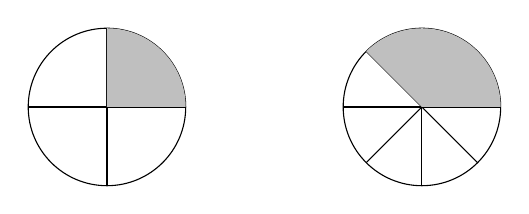
\begin{tikzpicture}
    % Primer círculo dividido en 4 partes, 1 sombreada
    \draw (0,0) circle (1cm);
    \draw (0,0) -- (1,0);
    \draw (0,0) -- (0,1);
    \draw (0,0) -- (-1,0);
    \draw (0,0) -- (0,-1);
    \fill[gray!50] (0,0) -- (1,0) arc (0:90:1) -- cycle;


    % Segundo círculo dividido en 8 partes, 2 sombreadas
    \draw (4,0) circle (1cm);
    \foreach \i in {0,45,90,135,180,225,270,315} {
        \draw (4,0) -- ++(\i:1);
    }
    \fill[gray!50] (4,0) -- ++(0:1) arc (0:90:1) -- cycle;
    \fill[gray!50] (4,0) -- ++(90:1) arc (90:135:1) -- cycle; % dos sectores
  
\end{tikzpicture}
\end{center}

¿Cuál es la suma de las dos fracciones representadas? Exprese el resultado como fracción simplificada.